
\label{sec:proposed-operational-workflows}
\textbf{Implementation boundary.} Figures in this section specify the \emph{target application design}. They are not additional completed experiments. The reproducible results in this manuscript concern the existing synthetic-data word-level TF--IDF and Linear SVM pipeline. The combined word/character representation and grouped sigmoid calibration were separately tested on existing synthetic development validation. Live probability reliability, class-dependent administrative review, case management and feedback-driven retraining still require independent implementation and measurement before production-readiness claims. Each diagram is placed immediately after the explanatory discussion of its named process; figure numbers are assigned by LaTeX captions rather than embedded in the graphics.

\subsection{Complaint Intake and Input Boundary}
The proposed resident-side form requires a \emph{Subject} and a \emph{Complaint Narrative}. If known, a date/time of occurrence and an approximate Purok/Sitio or landmark can be supplied as supporting context, without compulsory GPS or an interactive map. The narrative, not the user's name, phone number, assigned language tag or other metadata, is the primary input to the three-class SVM. The subject can be retained for case identification, but adding it to the classifier requires a separately documented experiment to preserve comparison with the recorded text-only baseline. The application should provide a confirmation and tracking reference and maintain authenticated access and lawful handling of resident information. The screenshots of Davao City Reports serve as a \emph{local interface precedent}, not evidence that its implementation has been replicated \cite{dcr,ra10173}.

The core scope excludes photo uploads, image classification, ensembles that combine images and text, automated determination of physical truth and mandatory GPS coordinates. Where urgent safety reports arise, an independent referral/escalation safeguard is recommended rather than allowing an ordinary three-class text prediction to prevent timely review. Such referral logic remains a system requirement, not an experimentally demonstrated function.

\subsection{NLP Preprocessing: Meaning-Preserving Candidate}
Figure~\ref{fig:op-nlp} specifies a proposed conservative NLP routine. A secure original can be retained for authorized processing while the model operates on a minimized copy with direct identifiers masked when appropriate. The depicted privacy-oriented operational routine uses Unicode NFC, whitespace normalization, lowercasing and limited cleanup; these are intended to standardize representation without discarding \emph{hindi}, \emph{wala}, \emph{no}, \emph{not}, relevant number expressions or incident descriptions. Generic stopword removal, stemming and lemmatization are excluded from this proposed routine to avoid meaning-altering changes to mixed-language complaints. The current reproducibility scripts use scikit-learn TF--IDF's text processing; the separately depicted privacy masking and normalization stages are not asserted to be fully implemented in those recorded experiments. The separately evaluated development candidate instead uses NFKC/casefold/whitespace and no identifier masking, as specified in Section~\ref{sec:candidate-final}; these preprocessing variants must not be interchanged silently. Any masking accuracy must be assessed because over-masking can remove useful context and under-masking can expose personal information \cite{ra10173,sklearnpitfalls}.
\begin{figure}[H]\centering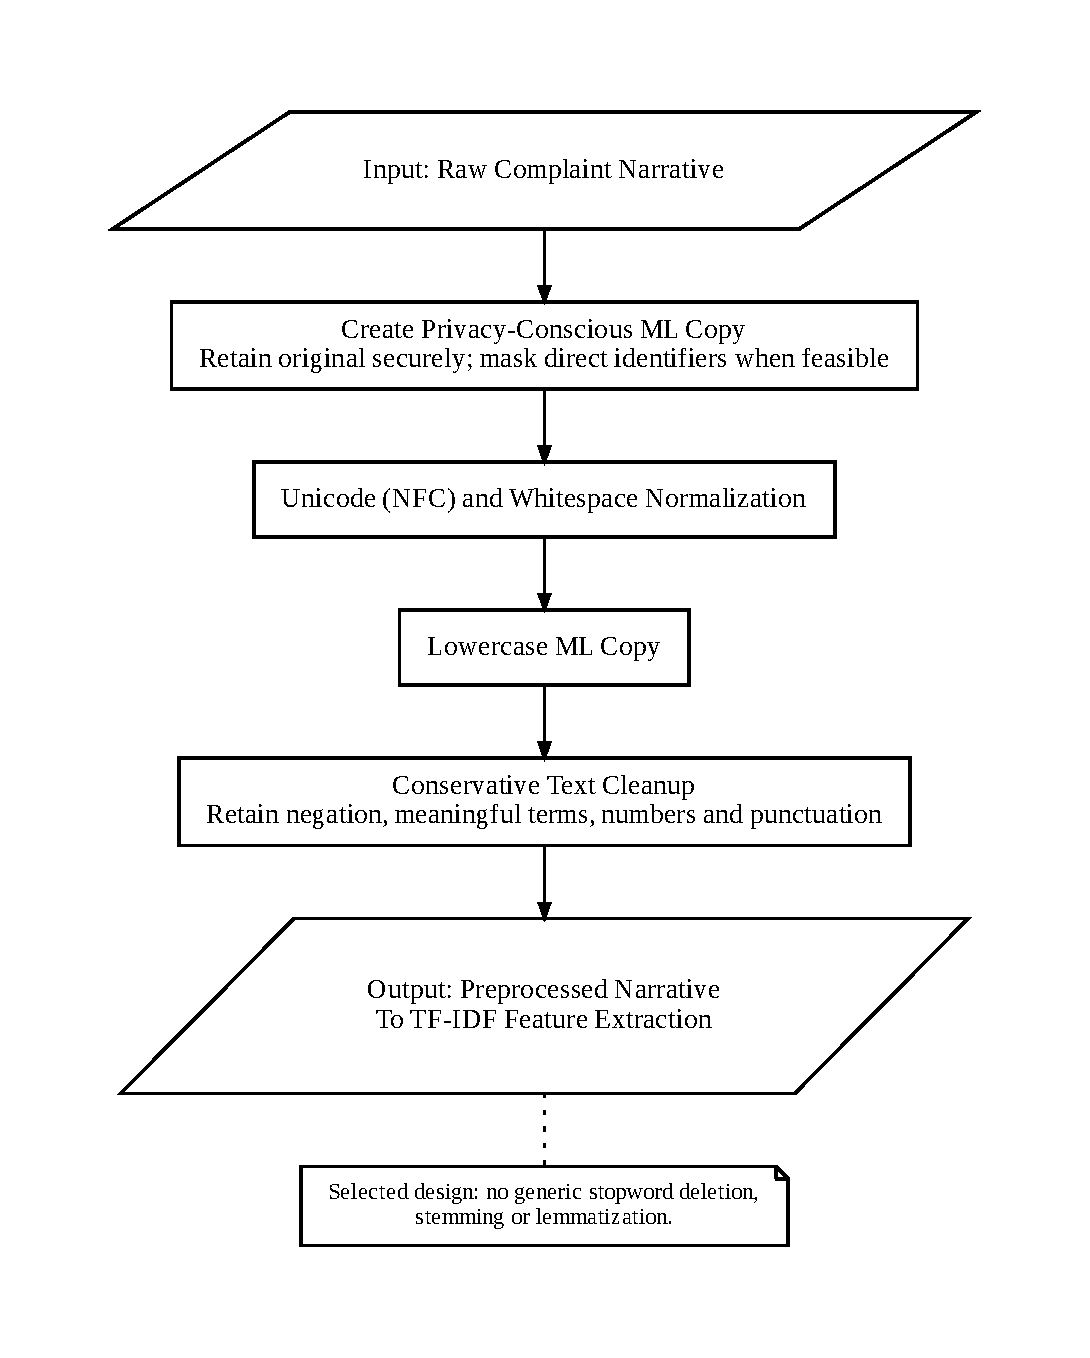
\includegraphics[width=.94\textwidth,height=.69\textheight,keepaspectratio]{figures/nlp_proposed.pdf}\caption{Proposed Natural Language Processing (NLP) preprocessing workflow for complaint narratives. Privacy-aware masking and normalization are target features, not measured preprocessing steps in the reported synthetic-data experiments.}\label{fig:op-nlp}\end{figure}

\subsection{TF--IDF Feature Extraction and Model-Level Consistency}
The recorded main SVM results used word-unigram TF--IDF, with a separately examined character-only ablation. Figure~\ref{fig:op-tfidf} describes the separately evaluated candidate using word unigrams and bigrams \emph{together with} character-within-word 3--5-grams. The resulting two sparse feature matrices are concatenated before classification. This combination is a \emph{separately evaluated development candidate}, not the verified configuration yielding the previously reported perfect within-generator score. In both configurations, vocabulary and inverse-document-frequency weights must be fitted within training partitions, never independently refitted on each new complaint. The deployed vectorizer and classifier should be versioned together \cite{sklearntfidf,sklearnpitfalls}.
\begin{figure}[H]\centering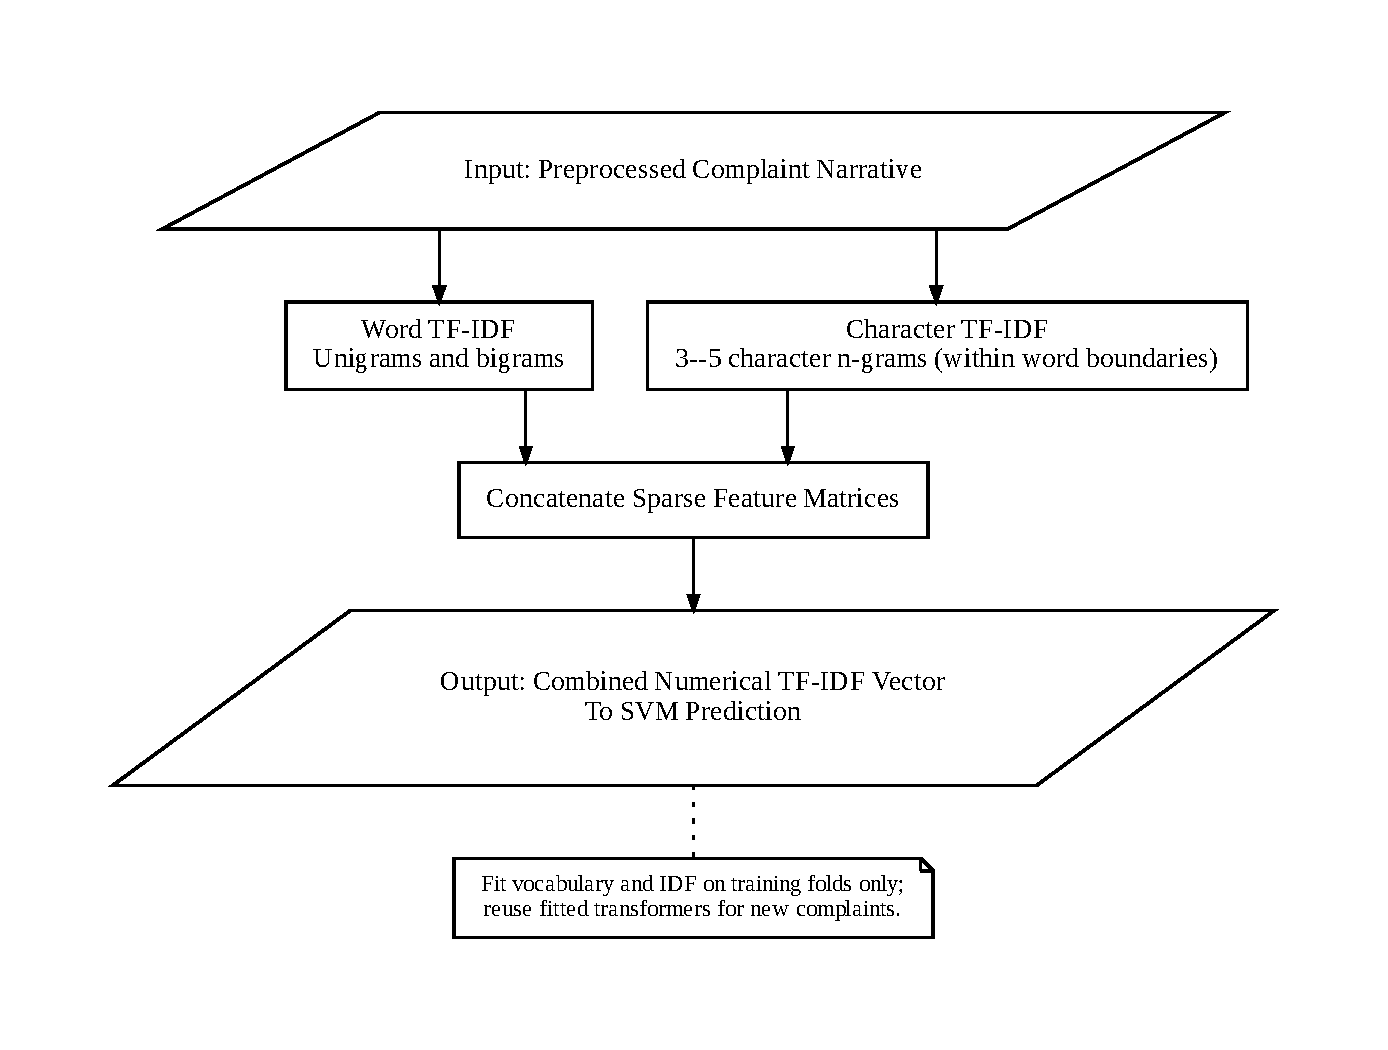
\includegraphics[width=.96\textwidth,height=.68\textheight,keepaspectratio]{figures/tfidf_proposed.pdf}\caption{Separately evaluated word--character TF--IDF candidate. Concatenation and grouped sigmoid calibration were evaluated on development validation and tied the original word-only SVM Macro-F1; operational deployment and external reliability remain unvalidated.}\label{fig:op-tfidf}\end{figure}

\subsection{SVM Training and Calibrated Prediction}
Figure~\ref{fig:op-svm} separates model fitting from inference. An offline Linear SVM is trained using authorized labeled data, with hyperparameter selection performed through training-only cross-validation. Before model probabilities can be described as \emph{calibrated}, an appropriate calibrator must be fitted using independent calibration folds or held-out training material, then evaluated for reliability. During inference, a new complaint is transformed by the saved compatible vectorizer and classified by the saved model; it is not used to fit the model. The three displayed class-probability quantities remain proposed operational outputs; the reference SVM is uncalibrated, while a separate candidate supplies synthetic development probability diagnostics in Chapter~4 \cite{sklearncalib,sklearnpitfalls}.
\begin{figure}[H]\centering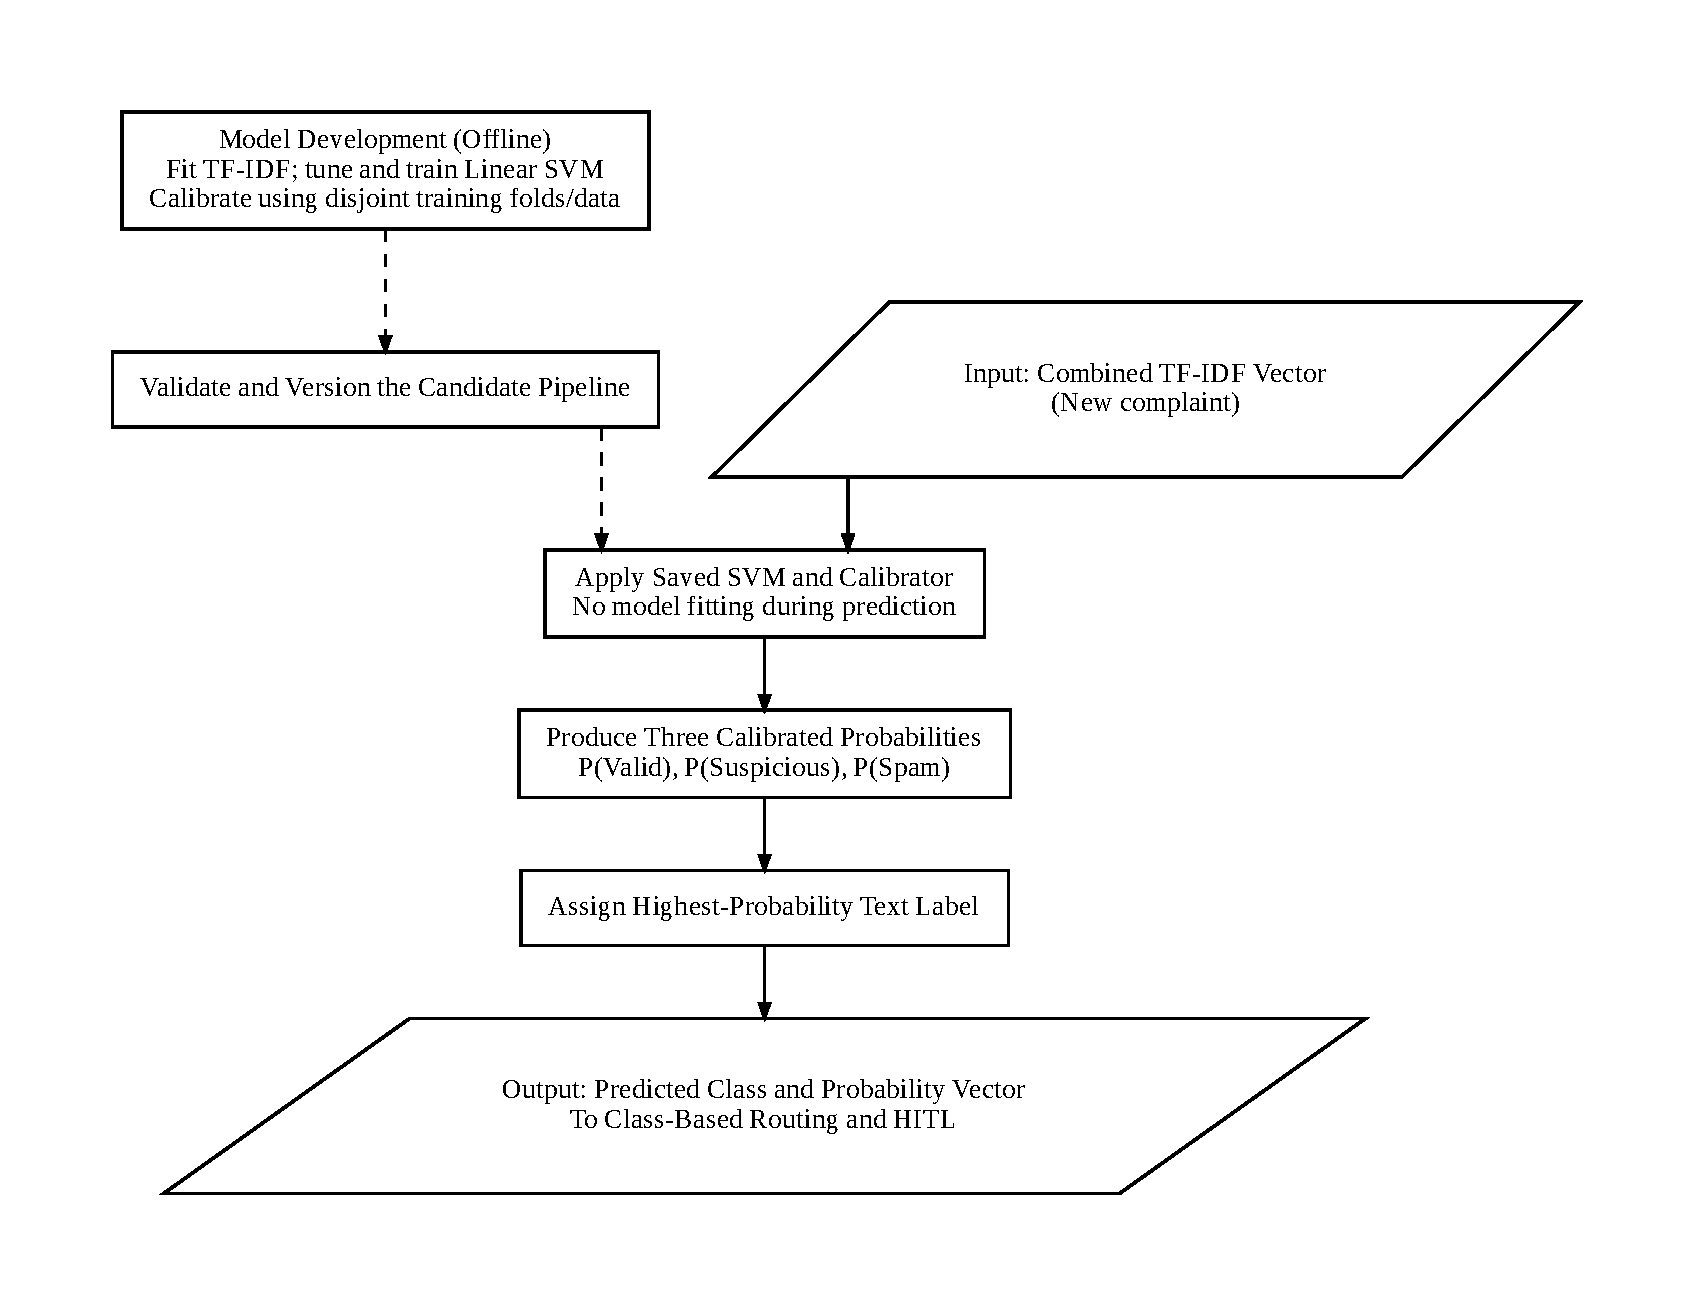
\includegraphics[width=.96\textwidth,height=.72\textheight,keepaspectratio]{figures/svm_proposed.pdf}\caption{Proposed support vector machine (SVM) model-development and new-complaint prediction workflow, with a separate probability-calibration requirement.}\label{fig:op-svm}\end{figure}

\subsection{Human-in-the-Loop Verification and Administrative Disposition}
The initial proposed routing rule is \emph{class-based}: predictions of Valid go directly to accepted-case handling, while predicted Suspicious or Spam are referred to the administrator for Human-in-the-Loop (HITL) review. Calibrated scores, once validated, may help \emph{prioritize} cases within the review queue; no numerical cutoff is fixed by this study. Under this design, an error that predicts Valid will not enter routine HITL, so a separately selected random audit of predicted Valid cases is necessary to estimate unobserved misclassifications. This is a proposed mitigation of the selective-label problem, not an implemented audit \cite{lakkaraju2017,madras2018}.

The administrator first examines the particular original text version and may confirm or correct its \emph{text label} to Valid, Suspicious or Spam. Separately, the administrator makes the \emph{disposition}: Accepted, Pending Clarification or Rejected with documented reason. Figure~\ref{fig:op-hitl} shows the decision boundary. A predicted Spam that was actually a clear complaint can be corrected to Valid and accepted; an incomplete original can remain Suspicious while external clarification permits administrative acceptance. No accepted case is automatically converted to a Valid training label, and no rejected case is automatically converted to Spam. A clarification request must be reassessed after a response or the applicable policy-governed response period; no invented universal deadline is imposed \cite{rottger2022,fleisig2024,franc2023}.
\begin{figure}[H]\centering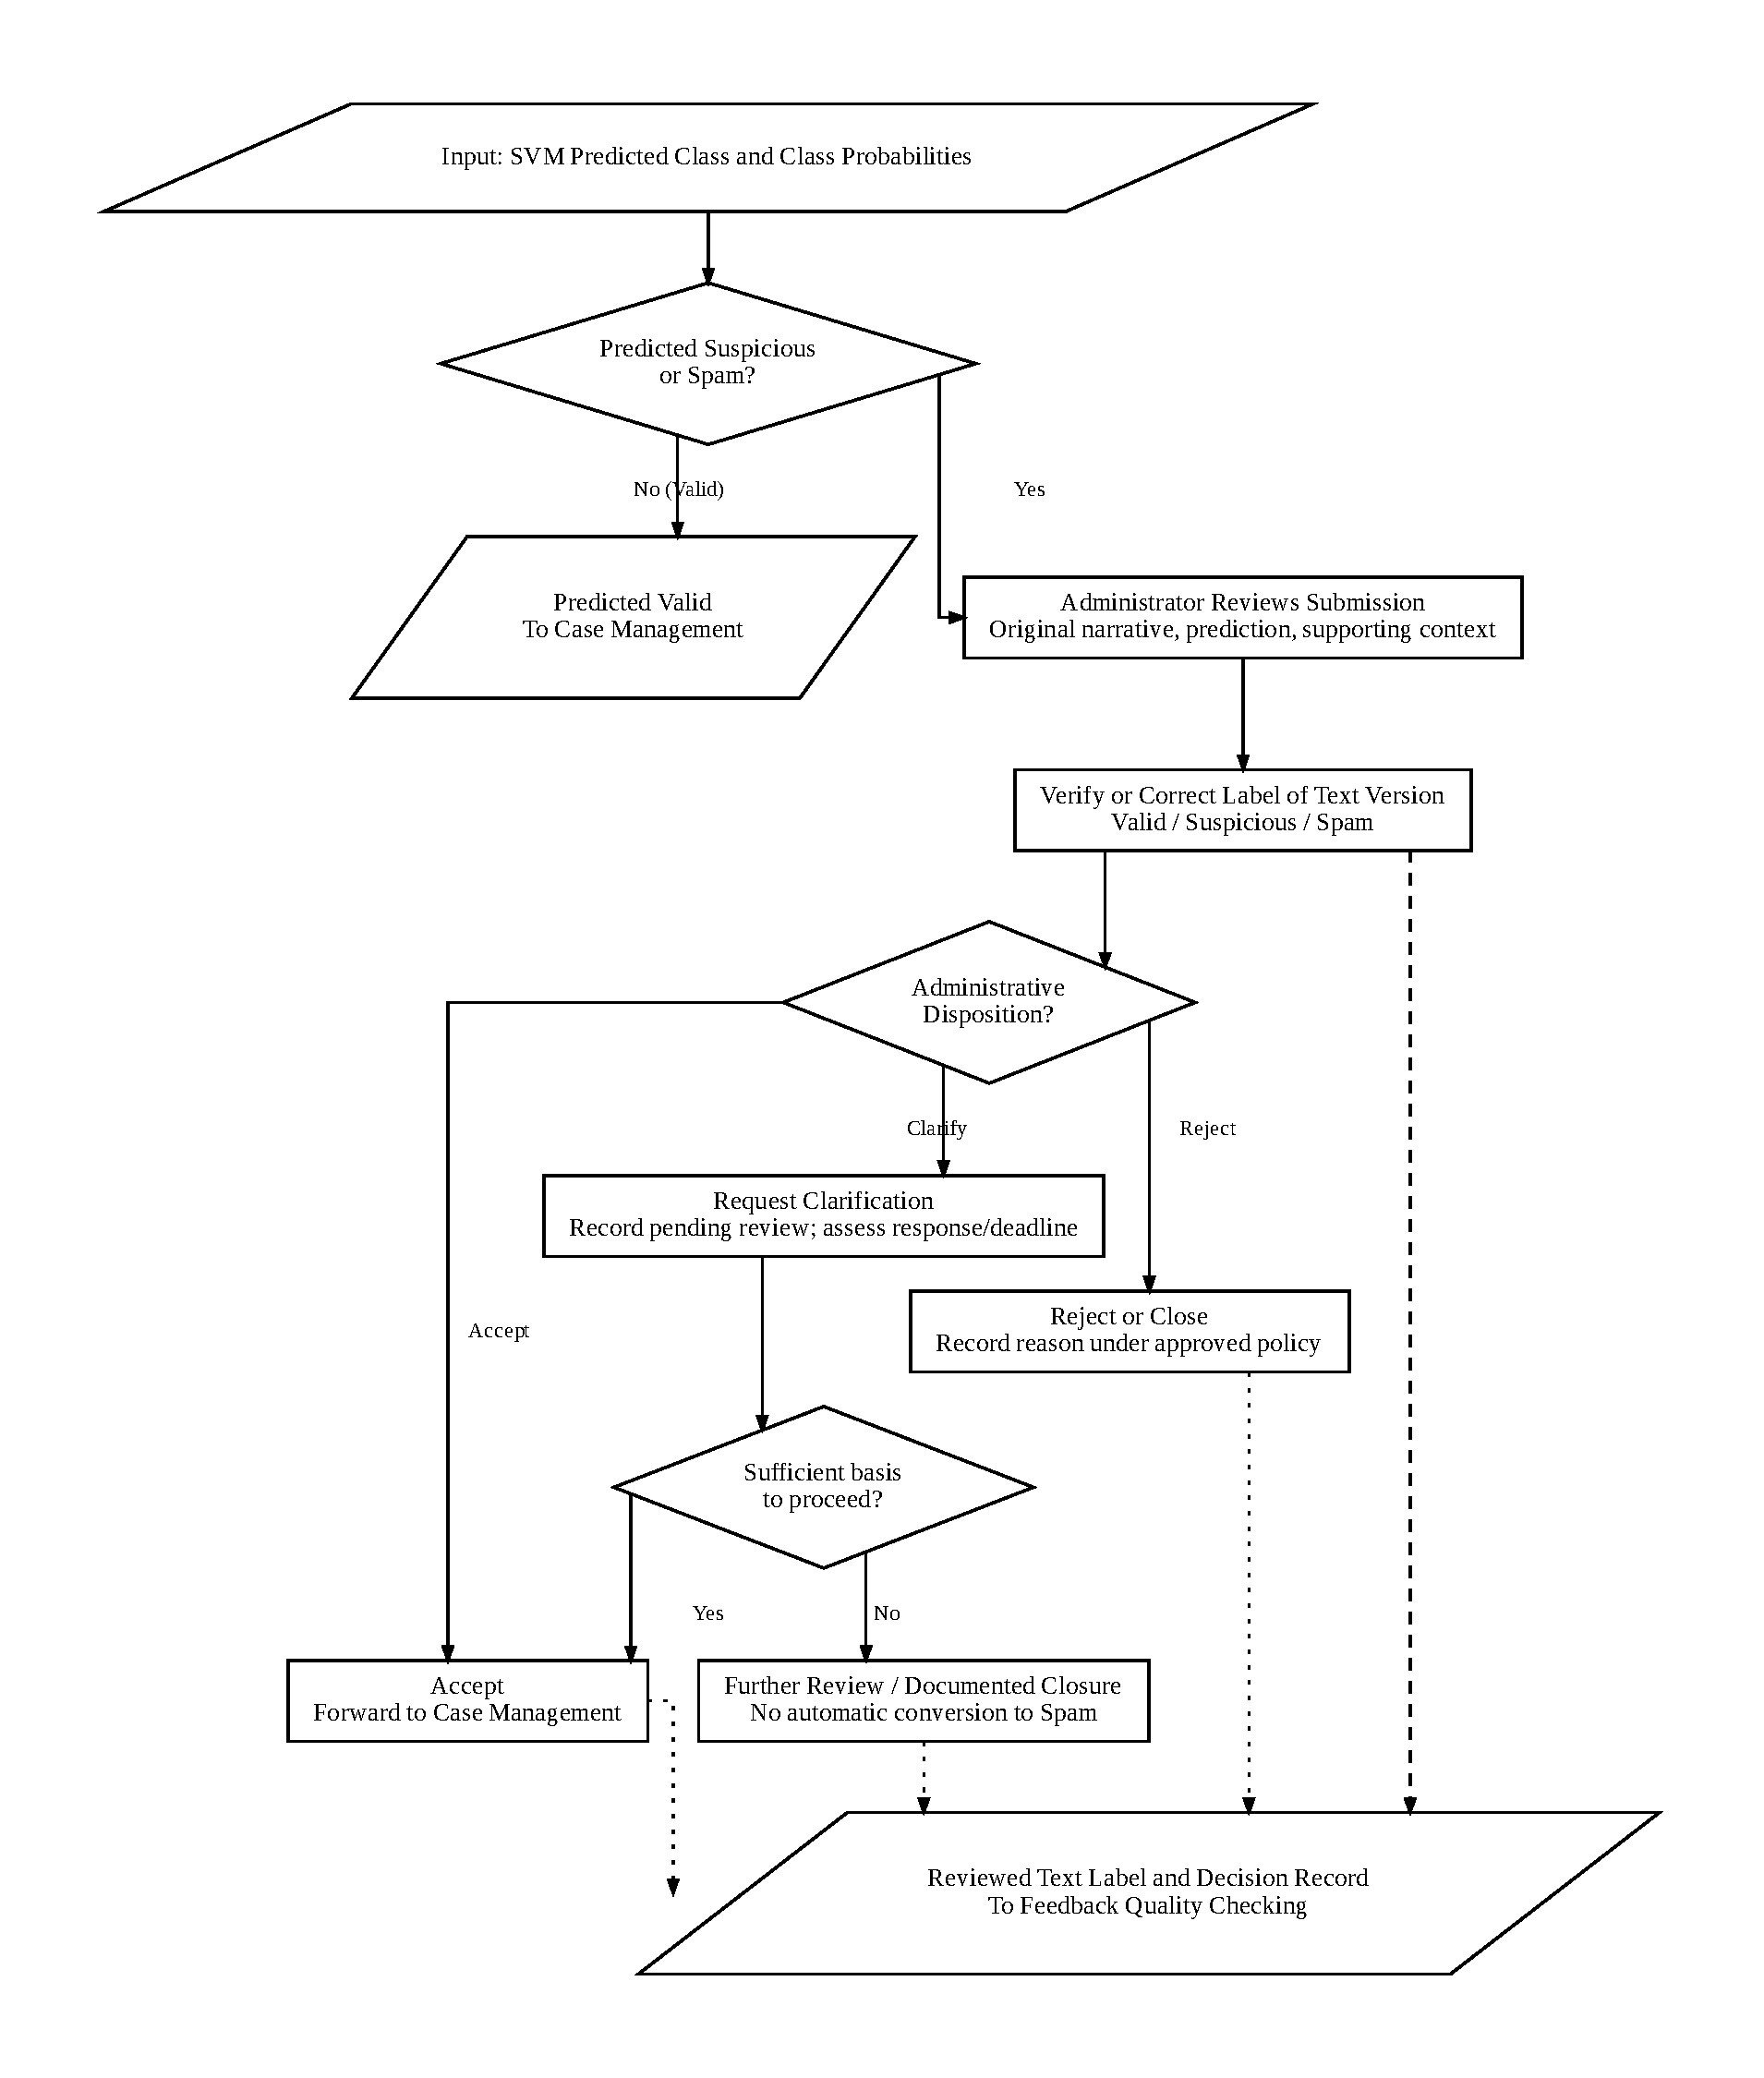
\includegraphics[width=.96\textwidth,height=.83\textheight,keepaspectratio]{figures/hitl_proposed.pdf}\caption{Proposed Human-in-the-Loop complaint review with distinct text-label verification and administrative disposition. Only predicted Suspicious or Spam enter routine HITL; direct Valid predictions proceed separately.}\label{fig:op-hitl}\end{figure}

\subsection{Nine Boundary Scenarios for Consistent Labeling}
Table~\ref{tab:op-boundary} operationalizes the ambiguous cases found in the consolidated evidence review. The text label applies to the \emph{narrative version}, not the independently investigated incident or the administrative case outcome. These are annotation and workflow rules to be validated by reviewers, not performance findings from an authentic dataset \cite{rottger2022,fleisig2024,li2023}.
\begin{longtable}{p{.39\textwidth}p{.23\textwidth}p{.29\textwidth}}
\caption{Proposed boundary-case labeling and administrative handling rules}\label{tab:op-boundary}\\
\toprule Scenario & Verified narrative label & Administrative handling\\\midrule\endfirsthead
\toprule Scenario & Verified narrative label & Administrative handling\\\midrule\endhead
Predicted Suspicious, but original text is already clear. & Correct to Valid. & Accept and route to case management.\\
Original is vague; resident supplies complete revision. & Original Suspicious; revised Valid. & Accept revised narrative; preserve both versions.\\
Original vague; independent evidence supports proceeding. & Original remains Suspicious. & May accept if authorized procedure permits.\\
Predicted Spam, but original is an actionable complaint. & Correct to Valid. & Accept; do not automatically reject.\\
Predicted Spam, but original is complaint-related and incomplete. & Correct to Suspicious. & Clarify; accept if sufficient information follows.\\
Predicted Suspicious, but content is promotional non-complaint material. & Correct to Spam. & Reject after human confirmation and record reason.\\
Text is clear but allegation has not been substantiated. & Valid as text. & Investigate or document outcome; truth not inferred by SVM.\\
Clear text later has legitimate administrative grounds for closure or rejection. & Valid as text. & Record grounds without changing text label.\\
Repeated similar submissions from one or several residents. & Label each version by its text. & Check duplicates and corroboration independently.\\
\bottomrule\end{longtable}

\subsection{Verified Feedback, Data Quality and Controlled Model Retraining}
Figure~\ref{fig:op-retrain} begins with versioned human-reviewed label records; it does not repeat the administrative Accept/Reject workflow. Records first undergo quality, duplicate, provenance, privacy and split-family checks. They are then accumulated in a verified-feedback pool. A periodic review of count, verified-class distribution, diversity, repeated errors and performance degradation determines whether a candidate training run is justified; the run requires authorization. Retraining is \emph{not triggered by each click} on an administrative button. An approved run consolidates the existing eligible training material and the new verified examples, refits the preprocessing and vectorization components, trains and recalibrates a candidate SVM, and evaluates it on a fixed independent validation protocol. A candidate that fails release criteria is archived without replacing the live model; a candidate that passes can be separately approved and versioned for future predictions \cite{figueroa2012,ghose2024,sklearnpitfalls,nist}.

The consolidated research review proposes cumulative increments of \emph{100, 250 and 500} verified examples as learning-curve checkpoints, with 1,000 only if feasible. They are \emph{research planning choices}, not empirically validated minimums or automatic deployment triggers. The baseline plus those three candidates are four conceptual model configurations, but cross-validation and calibration can require many additional fits. All variants of one case and related synthetic templates must remain grouped to prevent evaluation leakage. A small independent audit of predicted Valid cases should prevent the feedback pool from consisting solely of Suspicious/Spam predictions. Existing synthetic-data Macro-F1 scores cannot demonstrate that retraining on authentic complaints improves generalization \cite{figueroa2012,beatty2018,citovsky2021,ghose2024,lakkaraju2017}.
\begin{figure}[H]\centering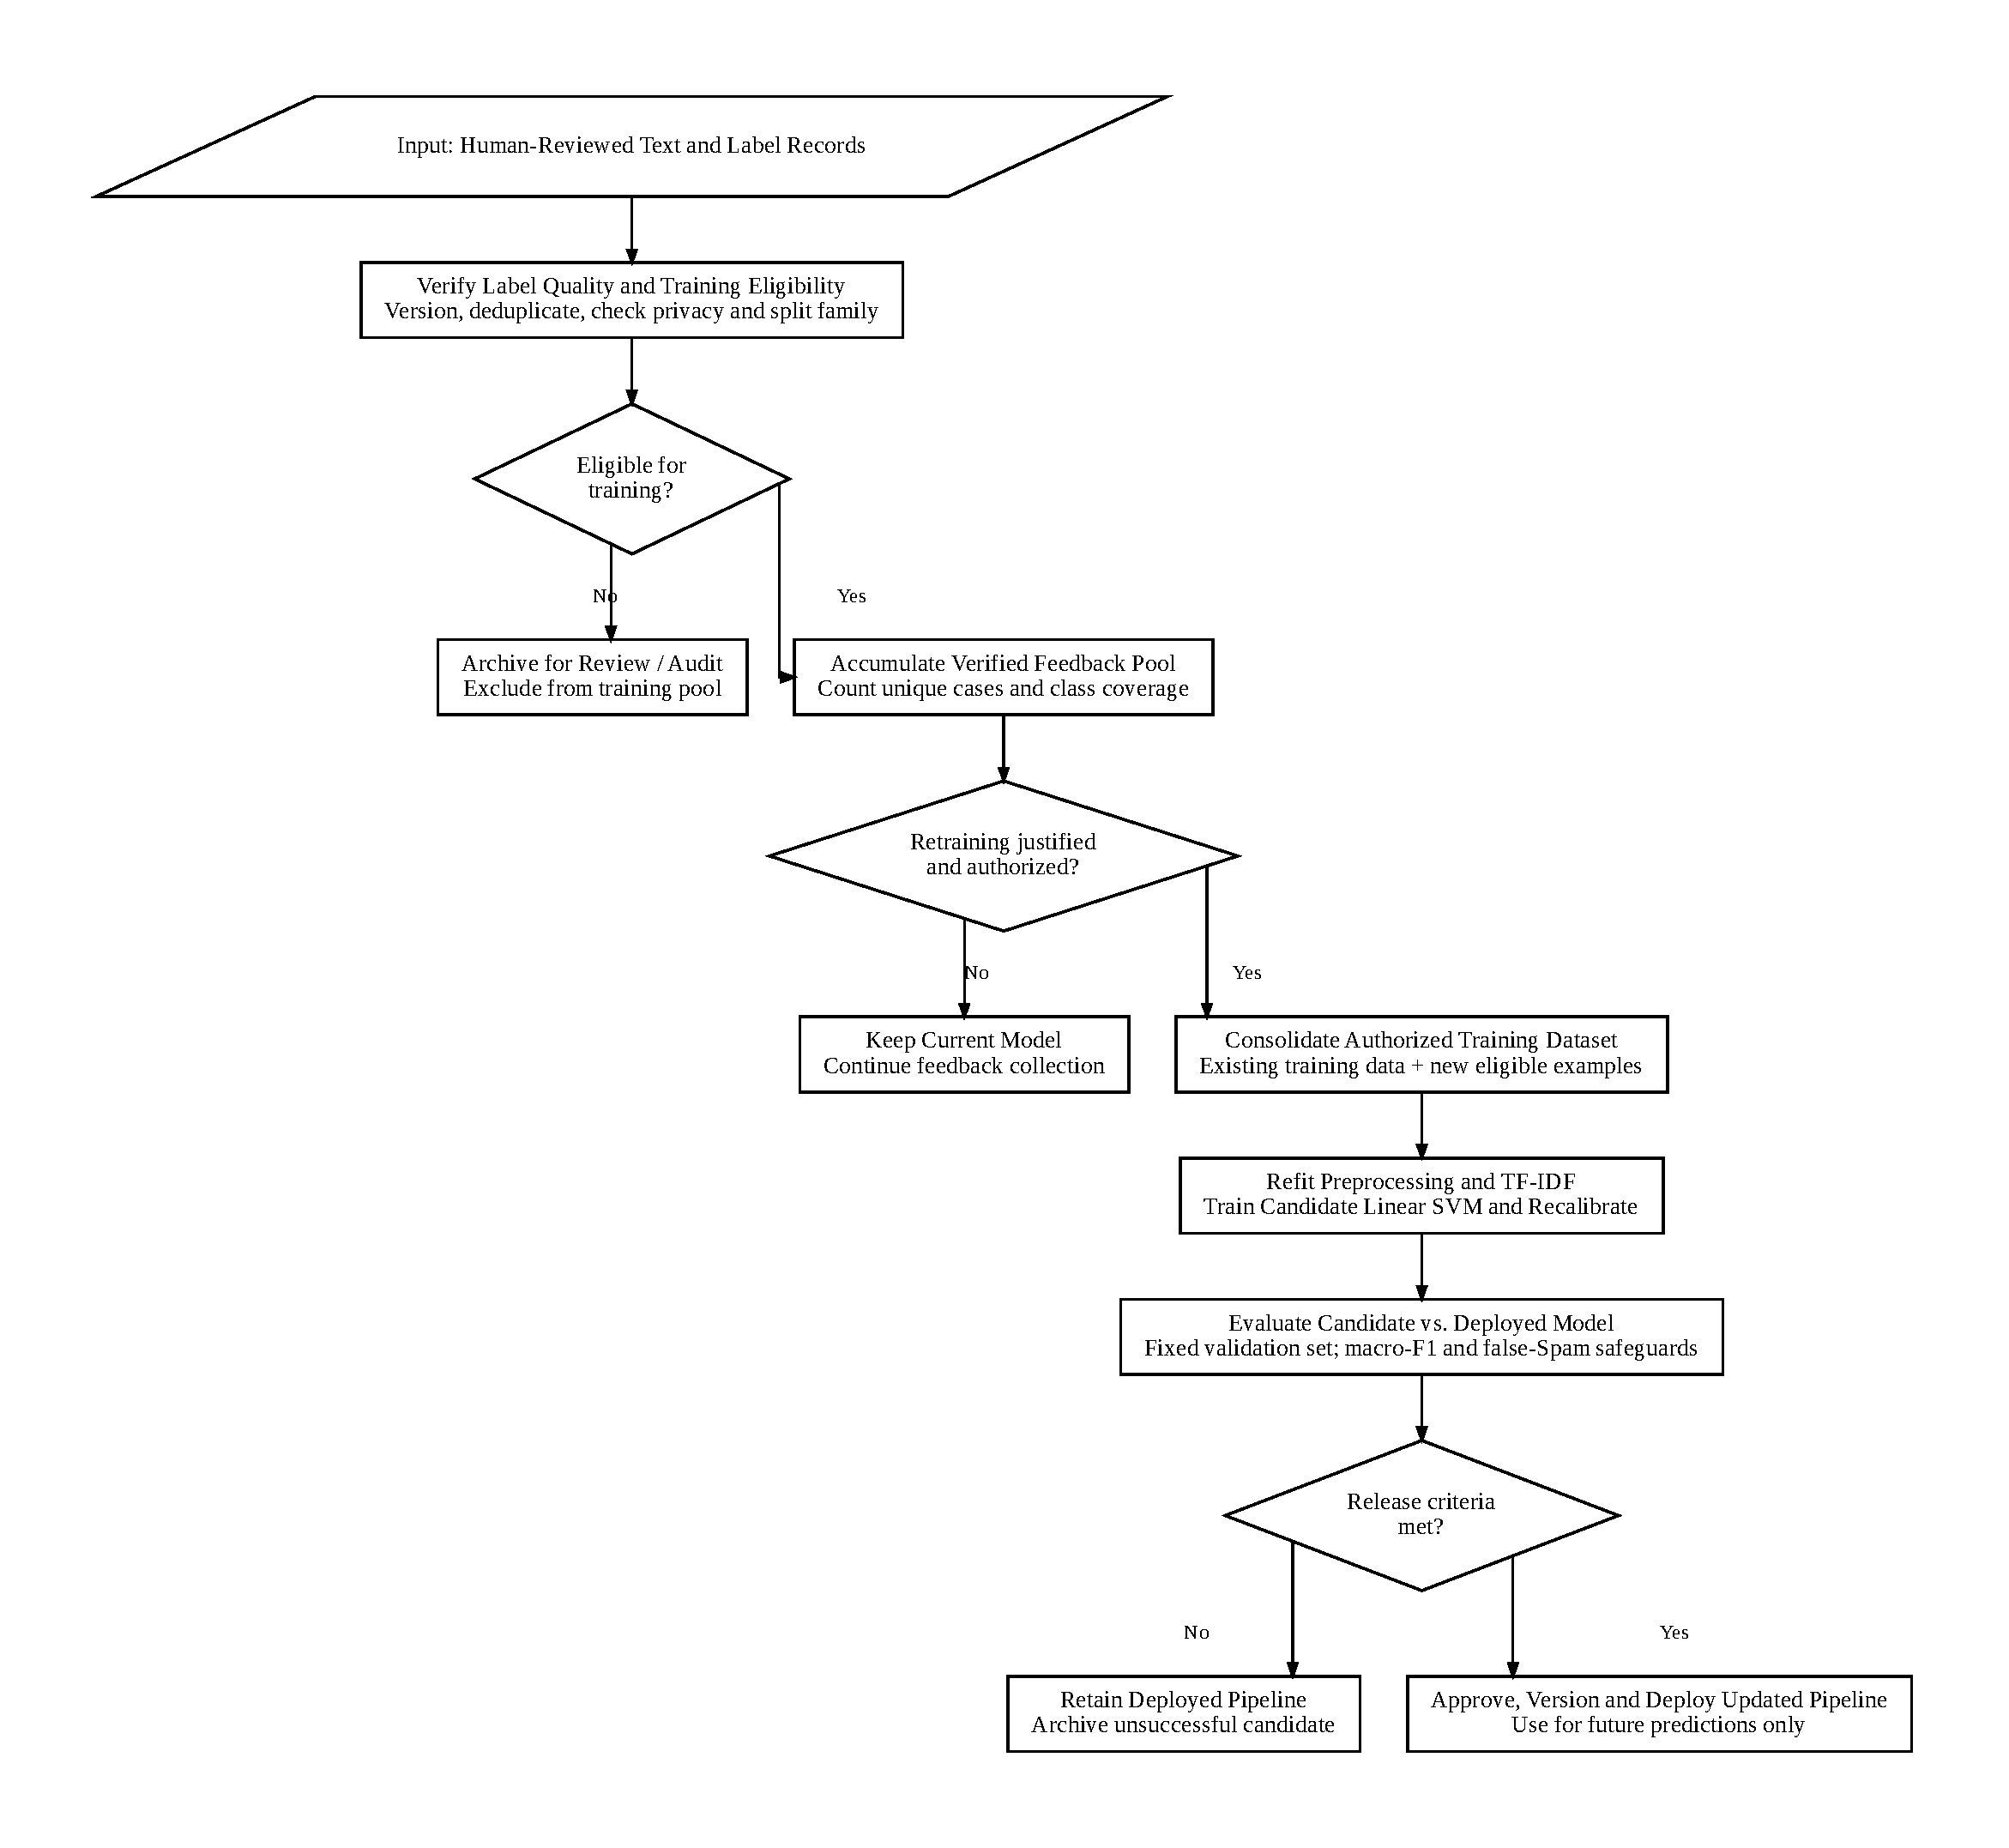
\includegraphics[width=.96\textwidth,height=.83\textheight,keepaspectratio]{figures/retrain_proposed.pdf}\caption{Proposed quality-checked human feedback and controlled batch retraining; training eligibility and deployment approval are separate decisions, and failure does not trigger infinite retries.}\label{fig:op-retrain}\end{figure}

\subsection{Accountable Complaint Case Management (Accepted Cases Only)}
The accepted-case workflow in Figure~\ref{fig:op-case} begins after the system accepts a predicted Valid narrative or an authorized administrator accepts a reviewed submission. The case receives a tracking identifier and a principal state of \emph{Unresolved}; designation of responsible staff, documented investigation and progress updates move the case to \emph{Ongoing}; independently checked completion allows it to become \emph{Resolved}. Records capture officer assignment, action timestamps, correspondence and supporting justification. \emph{Overdue}, \emph{Referred} and \emph{Reopened} are auditable events or flags, not additional SVM labels. If an action is unfinished, disputed or inadequately verified, the case returns to follow-up rather than being silently finalized.

This proposed administrative design is grounded in the distinction between public \emph{response obligations} and full incident resolution. Republic Act No.~6713, Section~5(a), addresses replies to public communications within fifteen working days; Republic Act No.~11032 and the relevant Citizen's Charter govern processing of covered services by complexity. The special 72-hour concrete-action standard associated with the national 8888 channel is \emph{not} a universal deadline for resolving every barangay incident. The application must store the locally applicable rule, permit reasoned referral/escalation and support resident disagreement. Davao City Reports provides a local precedent for tracking references, progress history and re-filing, not a claim that this proposed barangay implementation already meets its requirements \cite{ra6713,ra11032,eo8888,dcr}.
\begin{figure}[H]\centering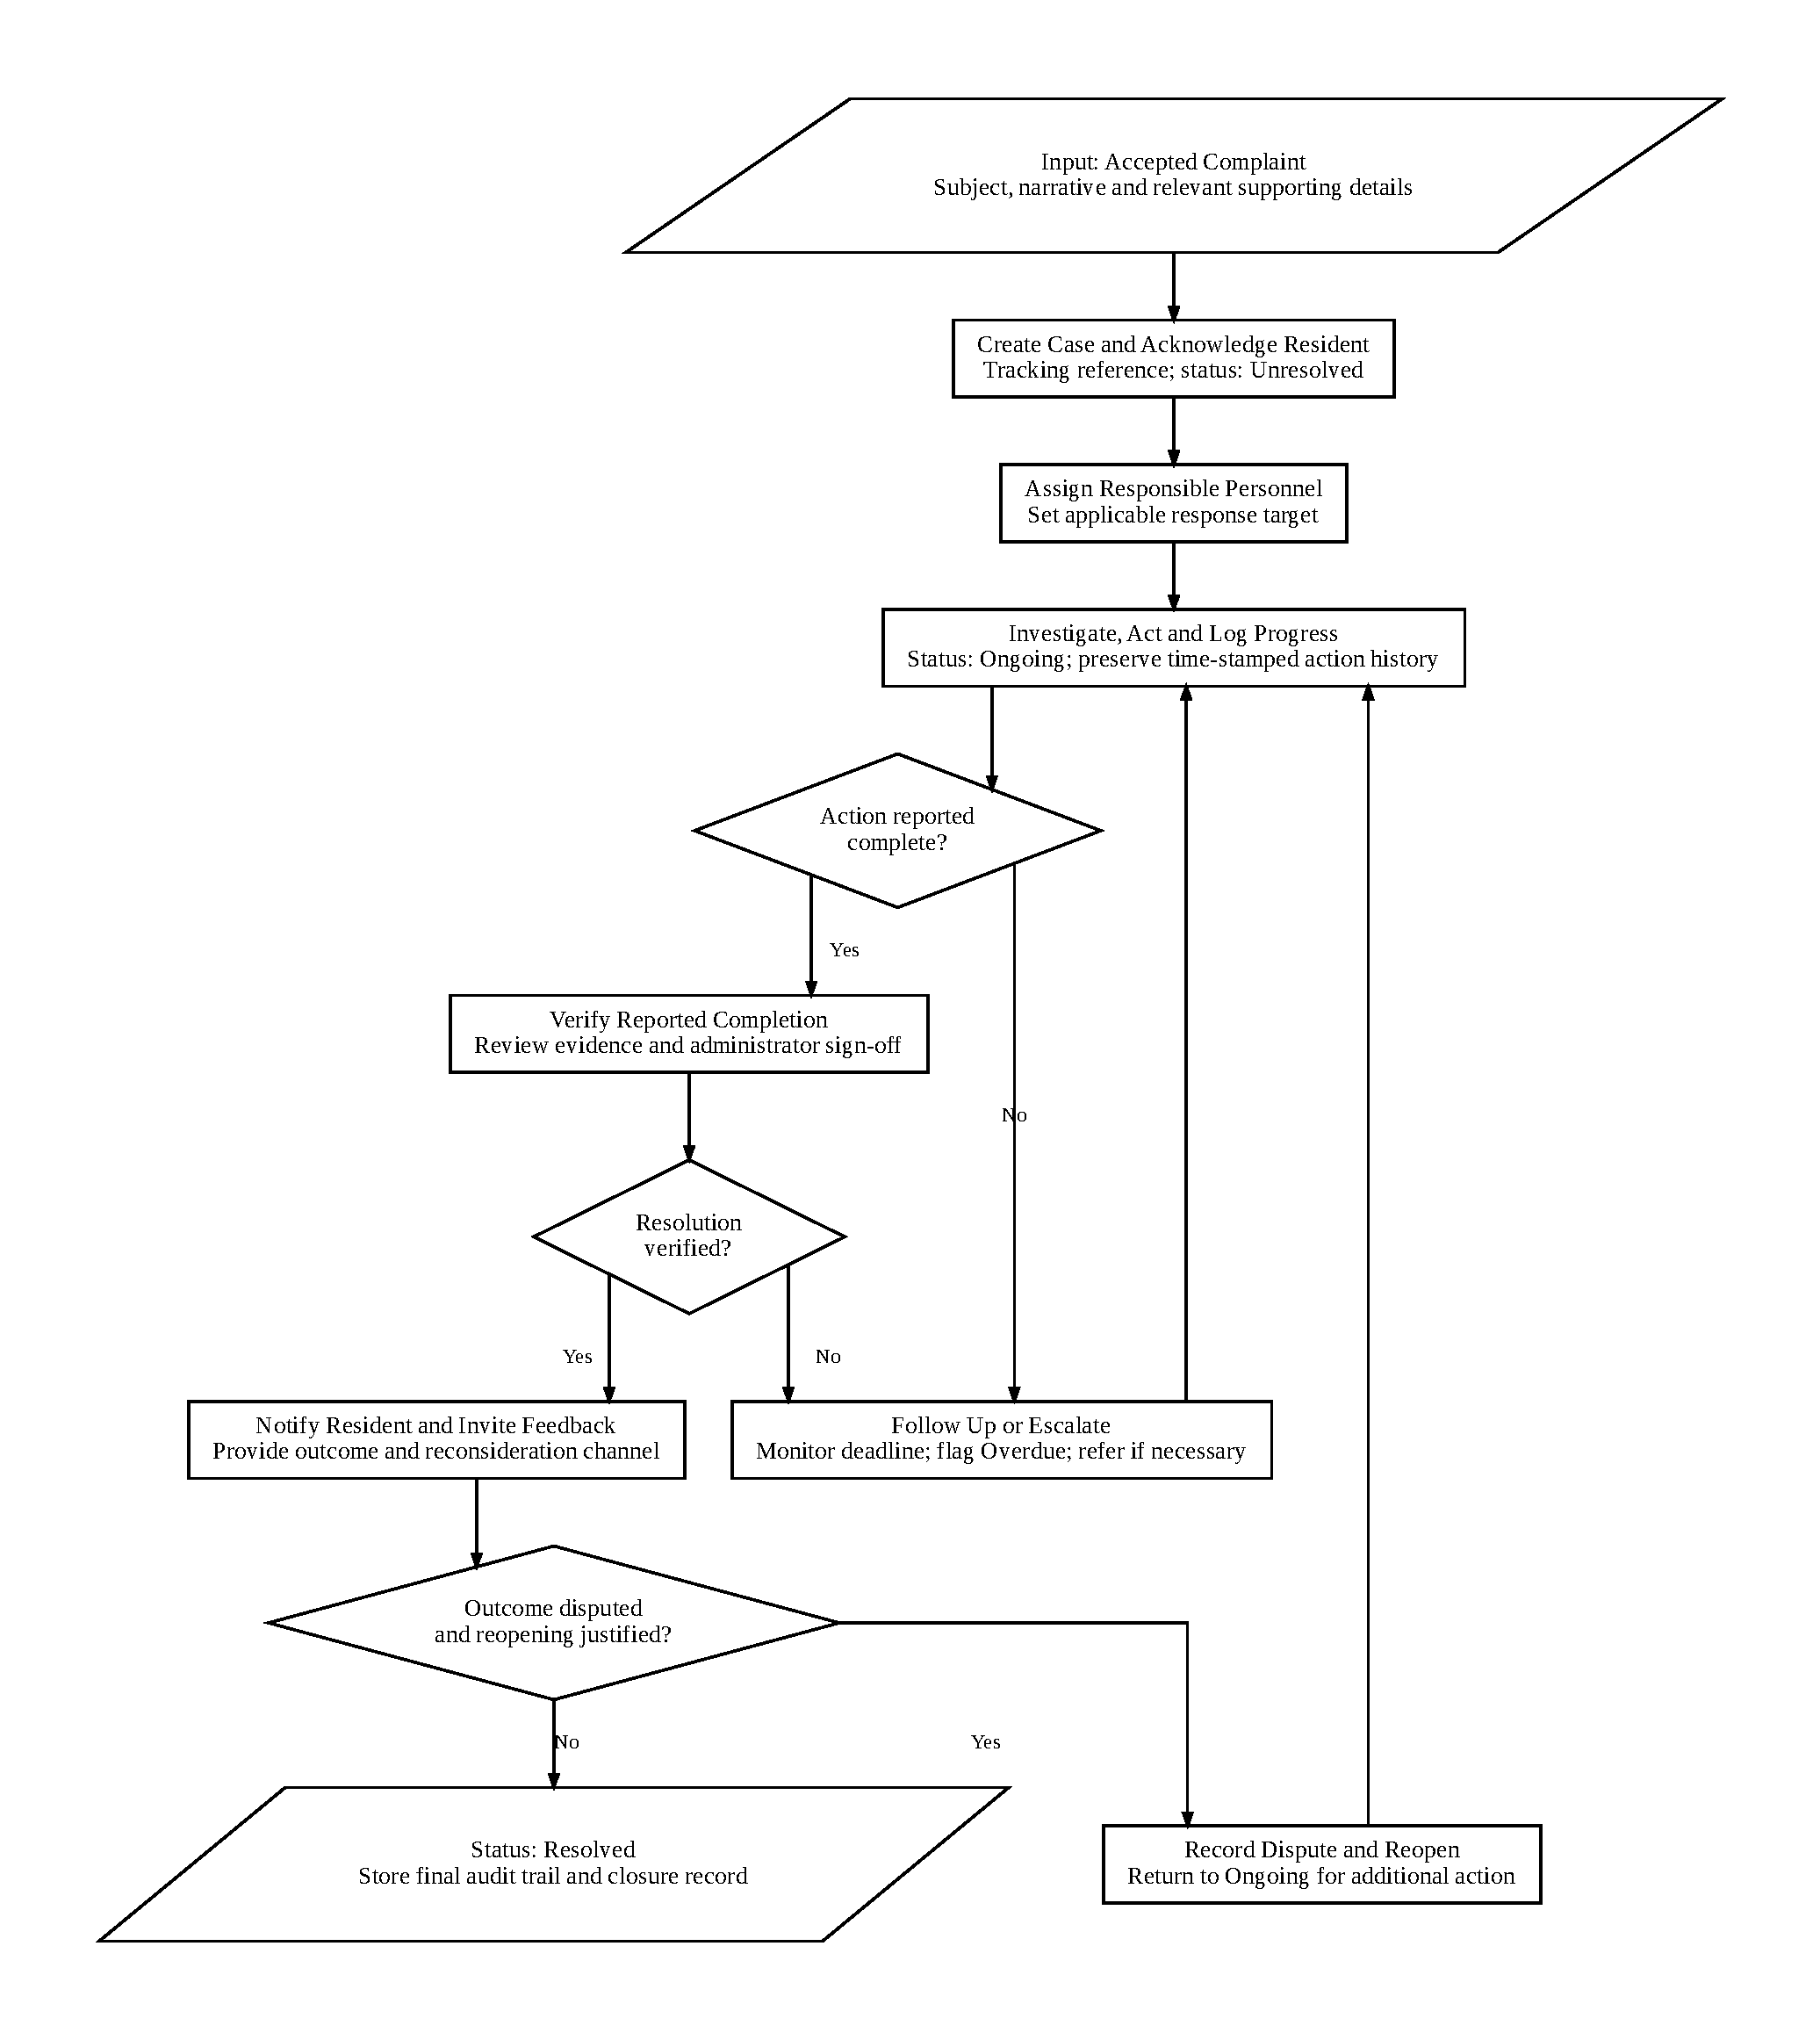
\includegraphics[width=.97\textwidth,height=.87\textheight,keepaspectratio]{figures/case_proposed.pdf}\caption{Proposed accountable complaint case management: accepted-case tracking, action logging, policy-based follow-up, completion verification, resident feedback and justified reopening.}\label{fig:op-case}\end{figure}

\subsection{End-to-End Integrated Complaint Workflow}
The integrated workflow in Figure~\ref{fig:op-integrated} links the previously described modules into one end-to-end account of proposed system behavior. A complaint narrative passes through conservative NLP preprocessing, saved word/character TF--IDF transformers and a calibrated SVM. Predicted Valid narratives proceed to accepted-case management; only predicted Suspicious or Spam narratives enter routine HITL for text-label verification and a separate administrative decision. Reviewed but non-accepted submissions retain a documented clarification or rejection outcome. \emph{Accepted} is an administrative state, not a replacement for the narrative label, while \emph{Resolved} is a later case-management state, not proof that an originally Suspicious sentence was Valid.

The diagram intentionally separates live case handling from the offline learning loop. Case records store assignment, action history, response deadlines and resolution outcomes, whereas versioned human-verified narrative labels are quality-checked before they can enter the training-feedback pool. Training a new TF--IDF--SVM candidate requires a justified and authorized retraining decision; the deployed classifier changes only after successful validation and release approval. In particular, neither an Accept click nor case resolution automatically updates model weights or training labels. These are proposed control boundaries, not additional observed results from the recorded synthetic-data baseline \cite{ra10173,rottger2022,sklearnpitfalls,nist}.
\begin{figure}[H]\centering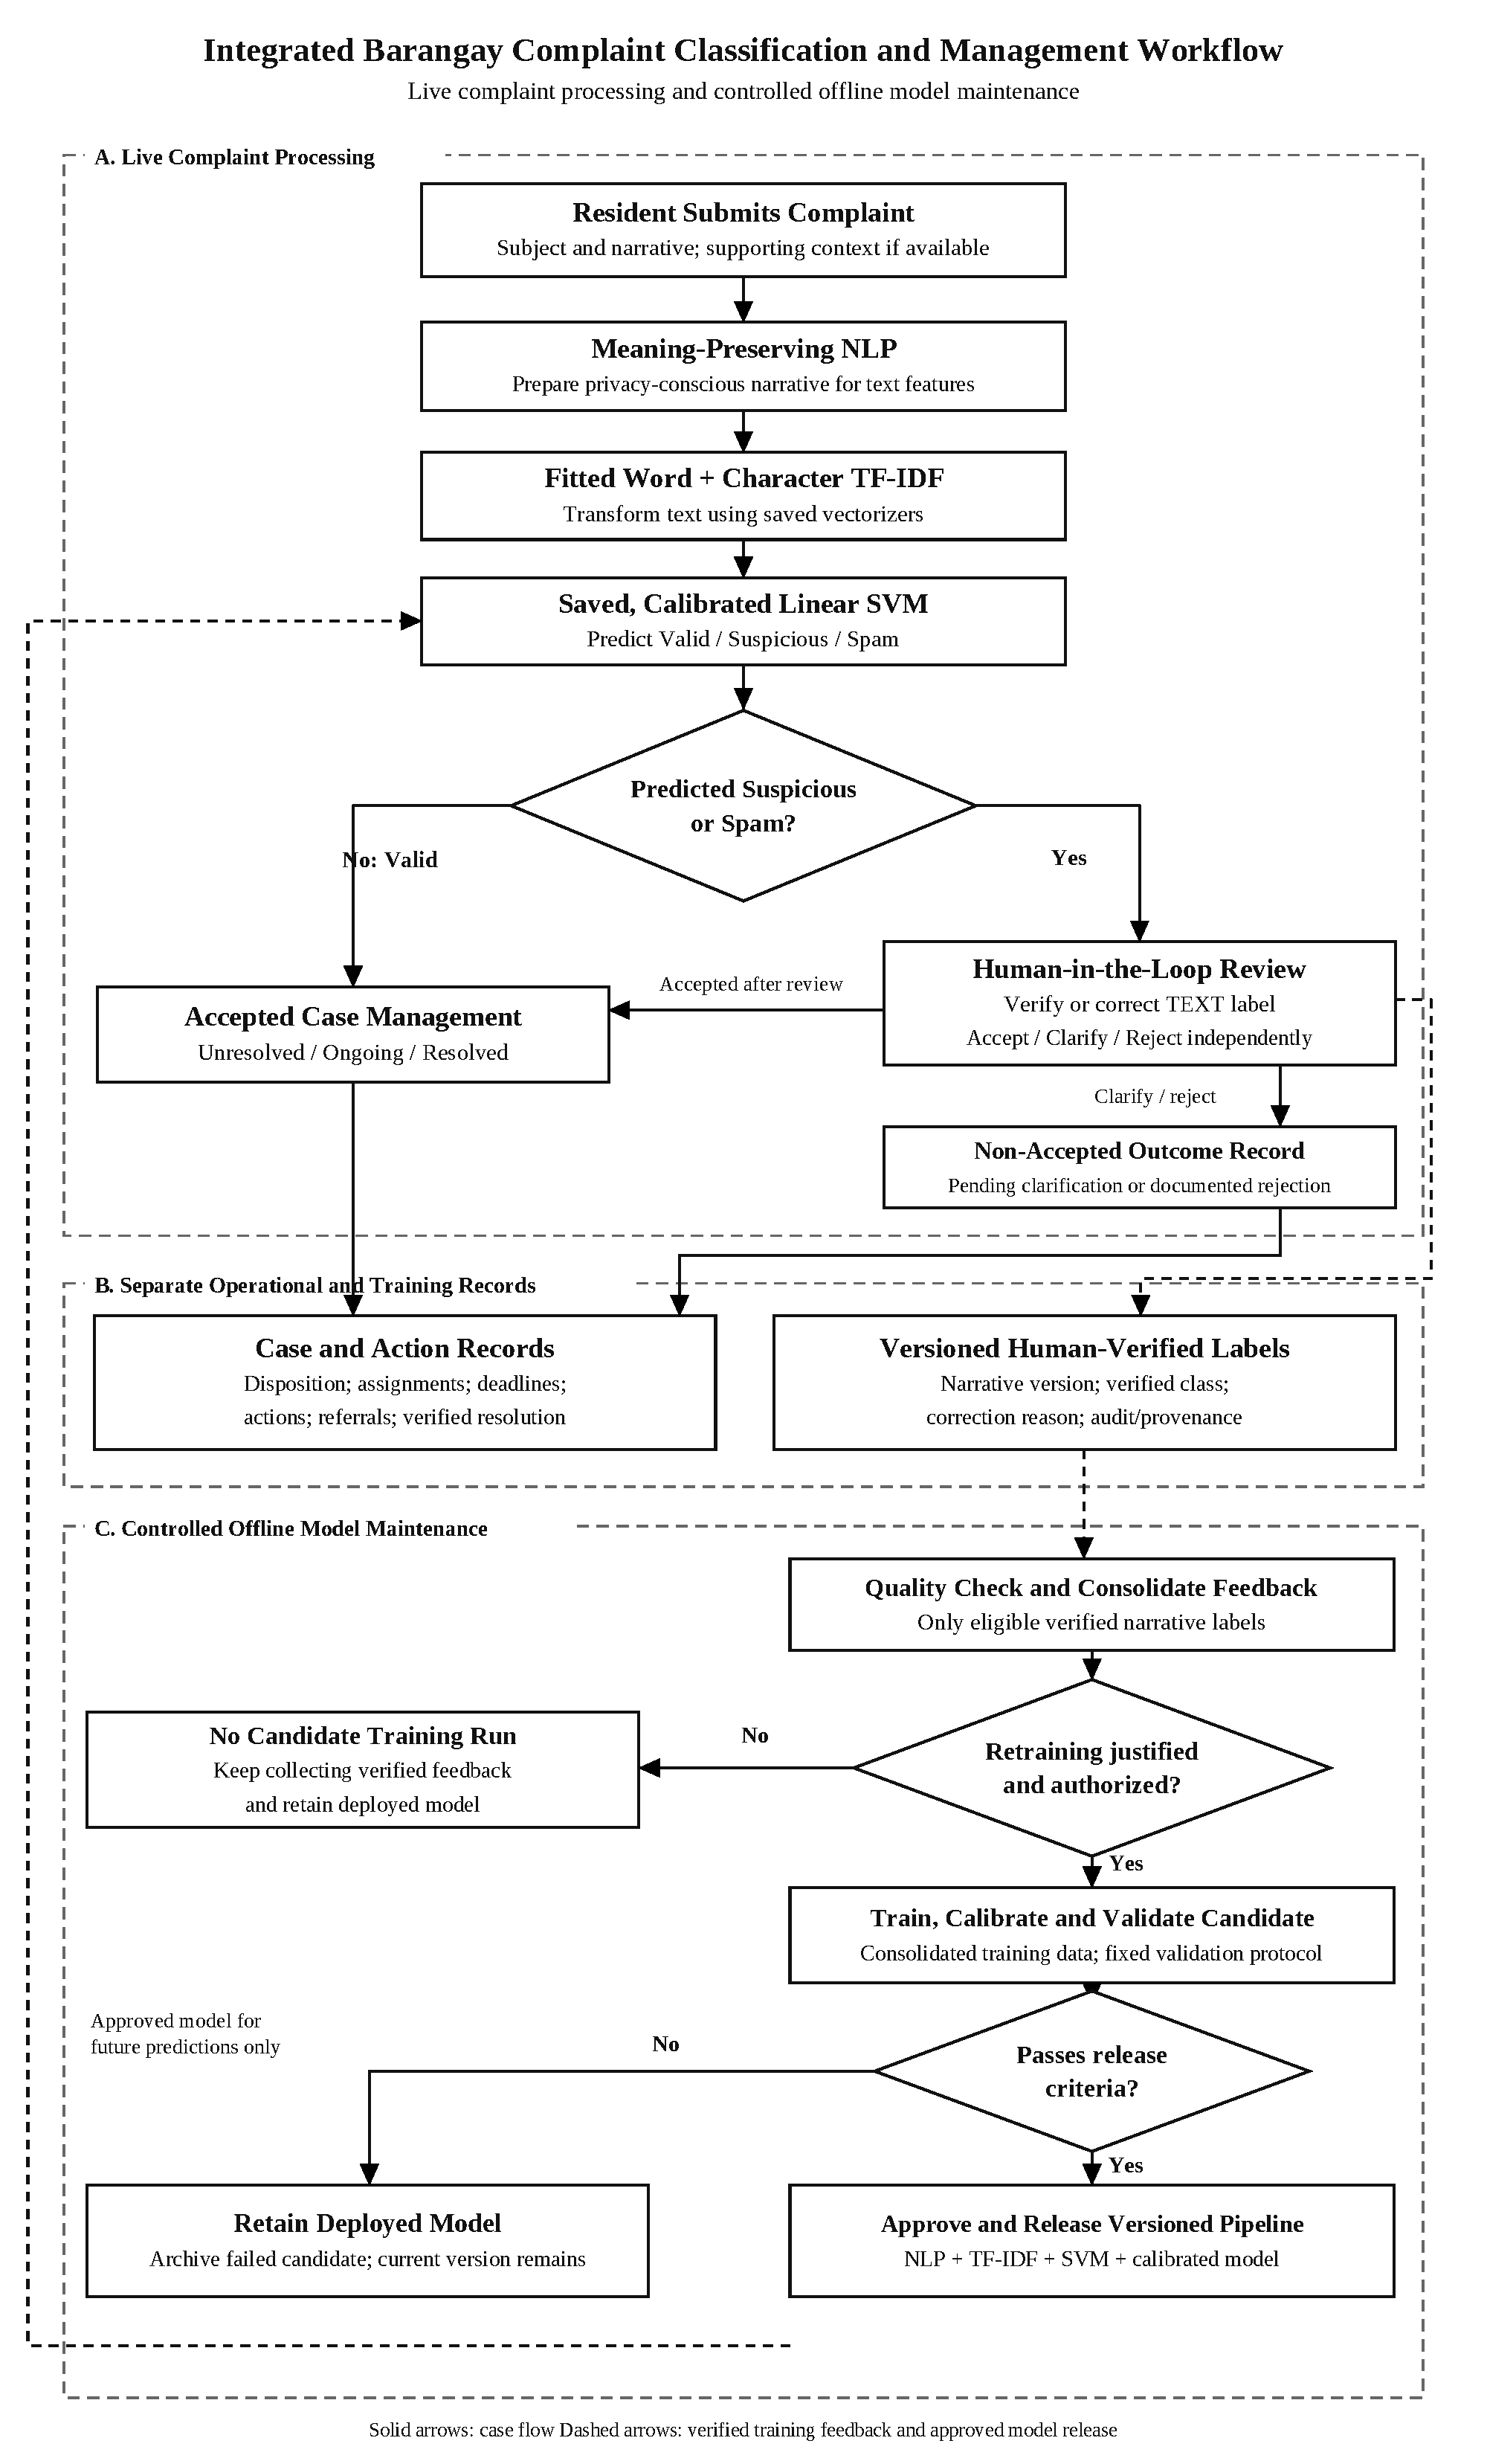
\includegraphics[width=.99\textwidth,height=.87\textheight,keepaspectratio]{figures/end_to_end_workflow.pdf}\caption{Proposed end-to-end integrated workflow connecting resident submission, NLP, TF--IDF, SVM, class-specific human review, accepted-case processing and approved offline retraining. Dashed arrows distinguish training-feedback and approved model updates from live complaint handling.}\label{fig:op-integrated}\end{figure}

\subsection{Software Component Integration and Data Boundaries}
After the end-to-end workflow, Figure~\ref{fig:op-system-integration} presents the complementary \emph{software component integration} and its access boundaries. The proposed resident portal and authorized administrator dashboard exchange data through a FastAPI application layer rather than calling the classifier or writing database records directly. The backend manages access checks, request validation, classification requests, tracking references, administrative actions and auditable case updates. Next.js/TypeScript, FastAPI/Python and PostgreSQL are the suggested application stack; the uploaded reproducibility evidence does not demonstrate deployment of these services.

The text-only inference service consumes the complaint narrative, applies the saved compatible preprocessing and TF--IDF transformations, and returns a saved calibrated SVM's proposed class probabilities. Predicted Valid follows the accepted-case service; predicted Suspicious or Spam enters administrator review. Reviewers may correct the \emph{text label} independently of Accept/Clarify/Reject decisions. Accepted cases and non-accepted submission outcomes share secured persistence but maintain different administrative states, while eligible verified narrative labels are stored as a \emph{distinct feedback dataset}. Later, an authorized offline candidate training run consolidates eligible training records, retrains the feature extractors and classifier, checks calibration and held-out validation, and releases a single versioned model bundle only after approval. The approved release path denotes an approved future inference version, never incremental training during complaint submission. The proposed design excludes photographic inputs and location maps from model inference and does not claim that a completed case is necessarily a Valid textual training example \cite{sklearnpitfalls,sklearncalib,ra10173,nist}.
\begin{figure}[H]\centering
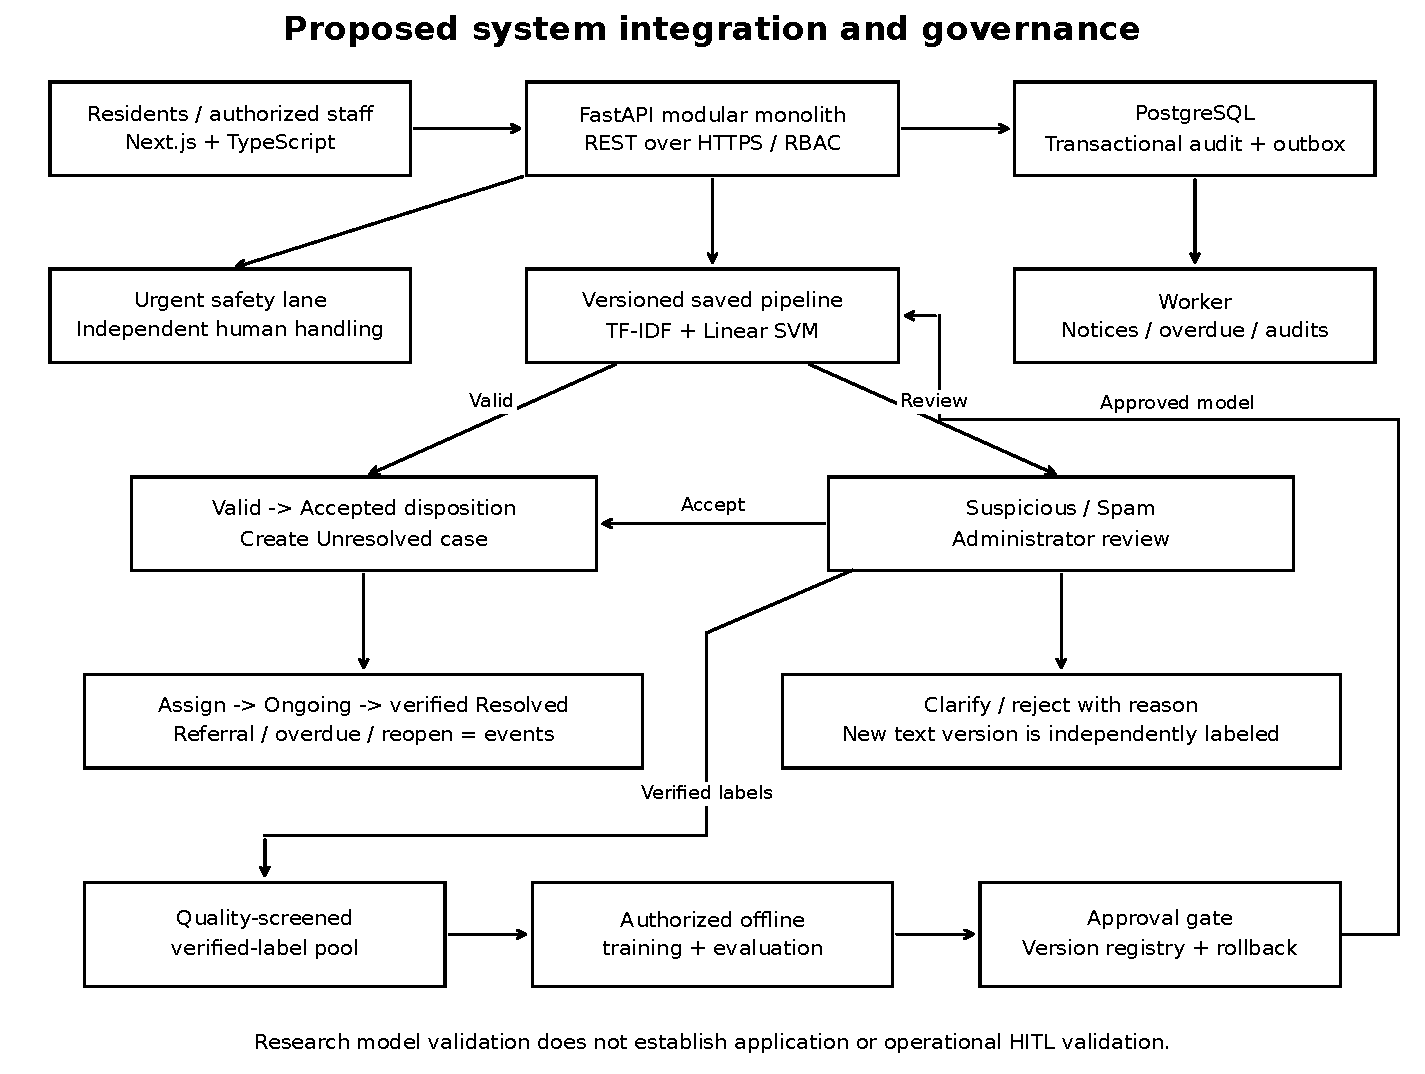
\includegraphics[width=.99\textwidth,height=.84\textheight,keepaspectratio]{figures/verified/system_architecture.pdf}
\caption{Proposed system integration architecture showing the resident and administrator interfaces, application API, text-classification service, HITL review, separate case and feedback records, and controlled offline model-release boundary. The component diagram specifies a target implementation, not a deployed or evaluated full-stack system.}\label{fig:op-system-integration}
\end{figure}

\subsection{Implementation and Evaluation Gates}
\begin{table}[H]\centering\small\caption{Evidence boundary and evaluation required for proposed extensions}\label{tab:op-evidence}\begin{tabularx}{\textwidth}{p{.29\textwidth}Xp{.24\textwidth}}\toprule
Component & What the supplied research currently supports & Required next evidence\\\midrule
24,000-row synthetic dataset & Fixed counts, partitions, metadata and researcher-generated texts; all review flags negative. & Human annotation and authentic external validation.\\
Word TF--IDF + Linear SVM & Recorded group-aware grid/CV and within-generator validation; test generalization remains limited. & Independent test beyond generator patterns.\\
Word + character combination & Reference reproduction and separate combined-feature development experiment. & Independent external comparison beyond the synthetic ceiling.\\
Probability calibration and HITL & Synthetic development calibration; HITL remains a proposed policy. & External probability reliability, reviewer agreement and Valid-sample audits.\\
Human-feedback retraining & Cumulative checkpoints and release-gate plan. & Verified feedback, fixed validation, approved candidate run.\\
Case management/accountability & Flowchart and local legal/interface precedents. & Implemented audit logs, deadlines, referral and resident tests.\\\bottomrule
\end{tabularx}\end{table}

\subsection{Detailed Full-Stack Implementation Plan}
The proposed architecture separates Next.js/TypeScript resident and administrator interfaces, FastAPI inference and workflow endpoints, and PostgreSQL records for versioned narratives, predictions, verified labels, dispositions and accepted cases. Object-scoped authorization, append-only histories, explicit state transitions, and model-release approval are required application controls. Figure~\ref{fig:op-system-integration} supplies the single software-integration overview; Figure~\ref{fig:verified-db} gives the complementary relational model. These are implementation plans, not validation of the existing SQLite/static-HTML prototype. Direct Valid routing records policy-based acceptance but never creates a human-verified label. Urgent human handling is independent of predicted class. The editable diagram sources and detailed schema are maintained in the repository documentation.
The relational design links immutable narrative versions to separate predictions and verified labels; accepted dispositions alone create cases. Append-only action and audit histories preserve the distinction between machine outputs and administrative decisions.

\begin{figure}[H]\centering
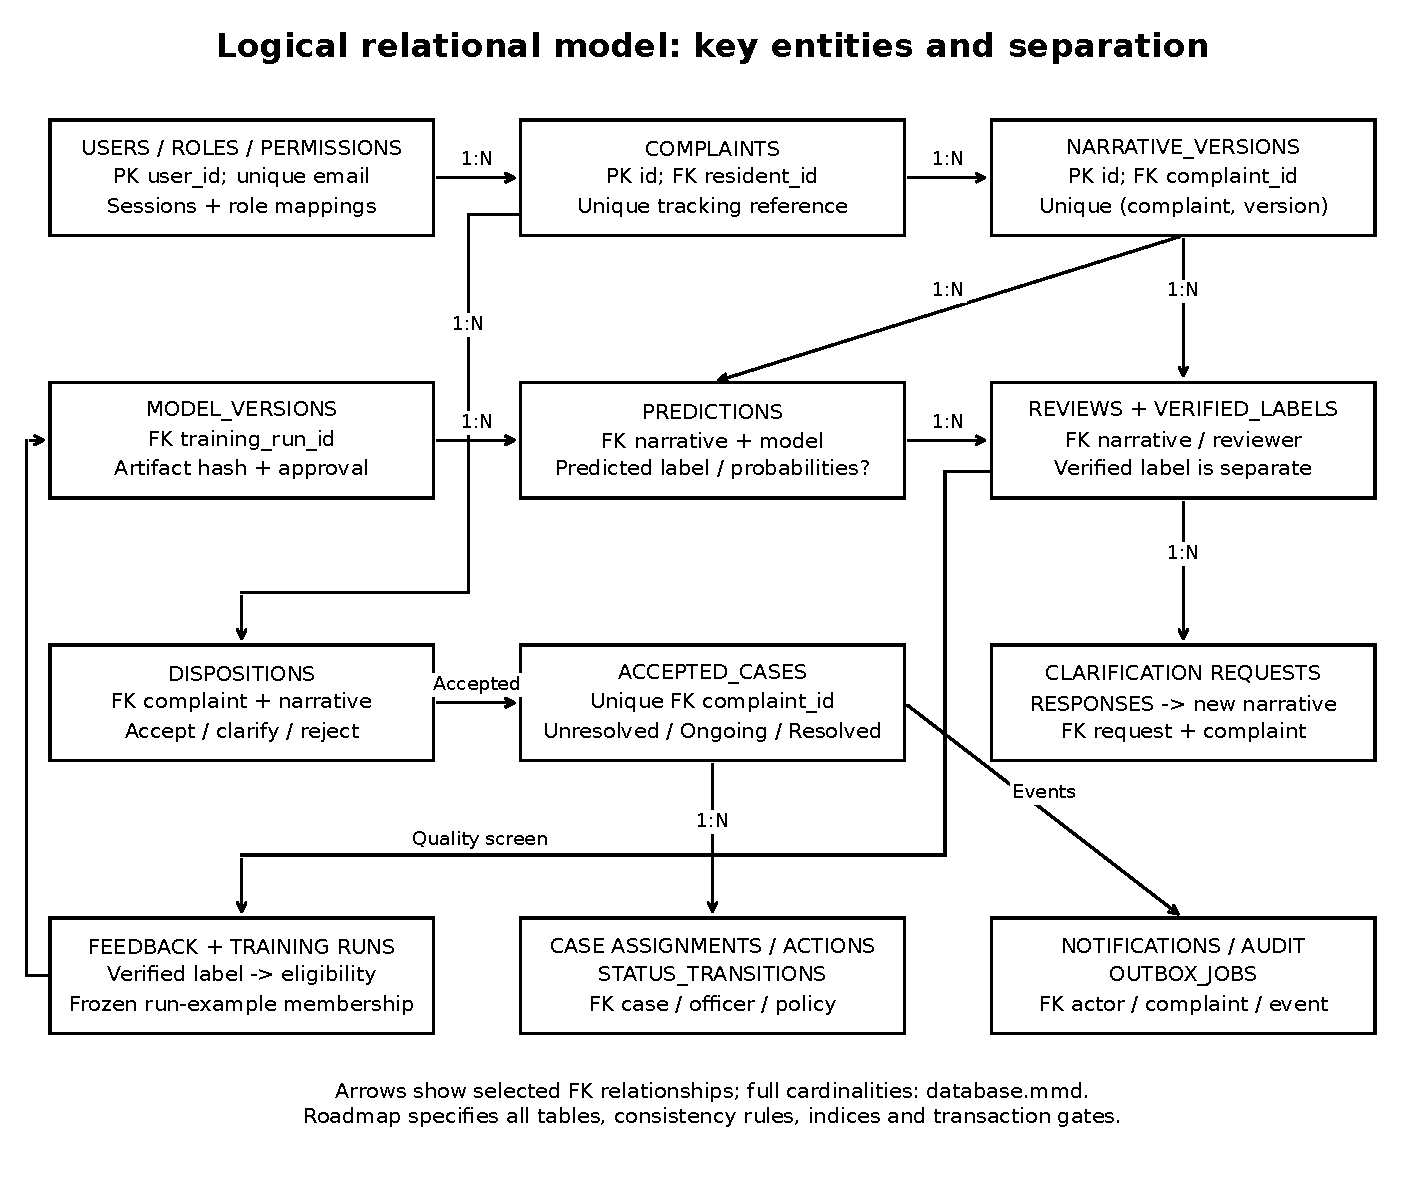
\includegraphics[width=.96\textwidth,height=.70\textheight,keepaspectratio]{figures/verified/database_overview.pdf}
\caption{Proposed logical relational overview; keys, constraints, indices and cardinalities are specified in the repository schema design.}\label{fig:verified-db}
\end{figure}
